\paragraph{La classe DriverCAN}

\begin{minipage}
    {\linewidth}
    \centering
    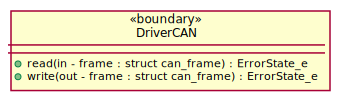
\includegraphics[width=0.50\linewidth]{../schemas/Conception_detaillee/classe_driverCAN.pdf}
    \captionof{figure}{Diagramme de classe de DriverCAN}
\end{minipage}

\subparagraph{Philosophie de conception \newline}

\medspace

La classe DriverCAN a pour rôle de communiquer avec le bus CAN. Elle est utilisée respectivement par les classes Sender et Sniffer pour envoyer et recevoir des trames sur le bus CAN. Cette classe utilise les SocketCAN pour communiquer avec le bus CAN et est donc dépendante de la bibliothèque can.h de Linux. 

\subparagraph{Description structurelle \newline}

\medspace

\textbf{Attributs :}
N.A.

\textbf{Services offerts :}

\begin{itemize}
    \item \textbf{write(in - frame : struct can\_frame) : ErrorState\_e} --- Opération qui envoie une trame sur le bus CAN. Elle renvoie un code d'erreur si l'envoi de la trame a réussi ou échoué.
    \item \textbf{read(out - frame : struct can\_frame) : ErrorState\_e} --- Opération qui lit une trame sur le bus CAN. Elle renvoie un code d'erreur si la lecture de la trame a réussi ou échoué.
\end{itemize}